% MRIxFields 2026 -- status deck #2.
% Numbers from reports/progress_report_2.tex, reports/spectral/alpha_summary.csv and
% "Baseline Experiment Logs.xlsx". Charts: python scripts/make_slide_figures.py --out-dir reports/figures
% Build: latexmk -pdf -bibtex- -interaction=nonstopmode progress_slides_2.tex
\documentclass[aspectratio=169,11pt]{beamer}

\usetheme{default}
\usepackage{lmodern}
\usepackage[T1]{fontenc}
\usepackage{amsmath}
\usepackage{amssymb}
\usepackage{booktabs}
\usepackage{array}
\usepackage{graphicx}
\usepackage{tikz}
\usetikzlibrary{positioning,arrows.meta}

\setbeamertemplate{navigation symbols}{}
\setbeamertemplate{footline}[frame number]
\setbeamercolor{frametitle}{fg=black}
\setbeamercolor{structure}{fg=black!70}
\setbeamerfont{frametitle}{size=\large,series=\bfseries}
\setbeamertemplate{itemize item}{\textbf{--}}
\setbeamertemplate{itemize subitem}{\textbf{\textperiodcentered}}

\definecolor{accent}{HTML}{1F4E79}
\definecolor{warn}{HTML}{9C2B2B}
\definecolor{good}{HTML}{2F6B3A}
\definecolor{neutral}{HTML}{8A8F98}
\newcommand{\hl}[1]{\textcolor{accent}{\textbf{#1}}}
\newcommand{\bad}[1]{\textcolor{warn}{\textbf{#1}}}
\newcommand{\ok}[1]{\textcolor{good}{\textbf{#1}}}

\newcommand{\parttag}[1]{{\scriptsize\textcolor{gray}{#1}}\par\vspace{0.3em}}
\newcommand{\gloss}[1]{{\footnotesize\textcolor{black!65}{#1}}\par}
\newcommand{\srcline}[1]{\vfill{\scriptsize\textcolor{gray}{#1}}}

% Presenter initials, top-right of each slide. One \ph{} per frame; replace PH per slide.
\newcommand{\ph}[1]{%
  \begin{tikzpicture}[remember picture, overlay]
    \node[anchor=north east, font=\tiny, text=black!40]
      at ([xshift=-3.5mm, yshift=-2.5mm]current page.north east) {#1};
  \end{tikzpicture}%
}

\newenvironment{airy}
  {\begin{itemize}\setlength{\itemsep}{0.8em}}
  {\end{itemize}}

\title{\bfseries MRI Field Translation}
\subtitle{Status, results, planned experiments}
\author{Berkin Deniz Kahya \and Furkan Yüceyalçın \and Racha Badreddine \and Ahmet Zelka}
\date{August 2026}

\begin{document}

\begin{frame}
  \titlepage
\end{frame}

% ============================================================ CHALLENGE =====

\begin{frame}{Challenge}
  \ph{F}
  \parttag{RECAP}

  \centering
  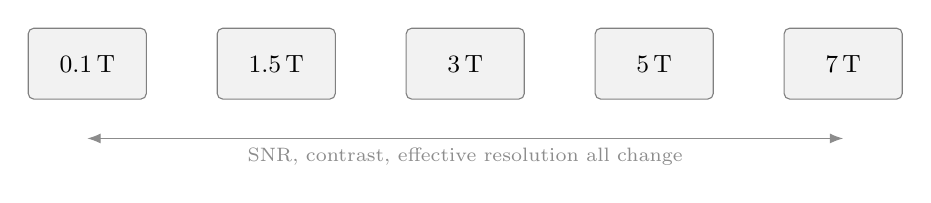
\begin{tikzpicture}[font=\small, >=Latex]
    \foreach \x/\lab in {0/{0.1\,T}, 2.4/{1.5\,T}, 4.8/{3\,T}, 7.2/{5\,T}, 9.6/{7\,T}}
      \node[draw=black!50, fill=black!5, rounded corners=2pt, minimum width=15mm,
            minimum height=9mm] at (\x,0) {\lab};
    \draw[<->, black!45] (0,-0.95) -- node[below, font=\scriptsize] {SNR, contrast, effective resolution all change} (9.6,-0.95);
  \end{tikzpicture}

  \vspace{1.4em}
  \raggedright
  \begin{airy}
    \item Translate brain MRI between field strengths. Three contrasts: T1W, T2W, T2FLAIR.
    \item 2500$+$ unpaired retrospective cases, 600 paired prospective cases, multi-centre.
  \end{airy}
\end{frame}

\begin{frame}{Tasks}
  \ph{F}
  \parttag{RECAP}

  \centering
  \resizebox{\linewidth}{!}{%
  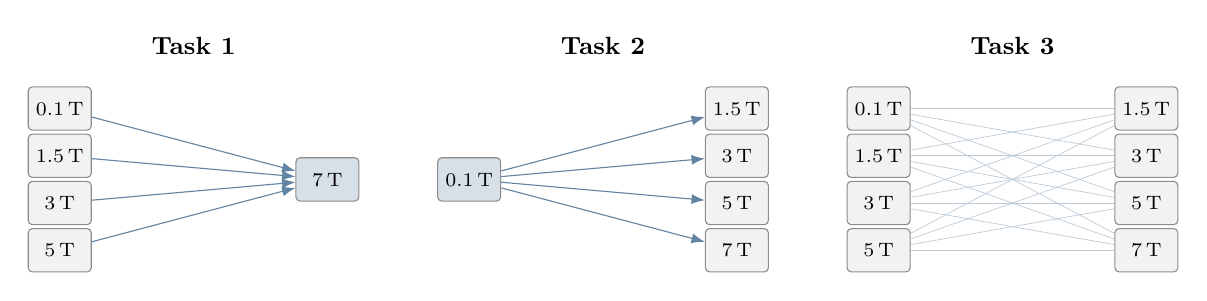
\begin{tikzpicture}[font=\scriptsize, >=Latex,
    f/.style={draw=black!45, fill=black!5, rounded corners=1.5pt, minimum width=8mm,
              minimum height=5.5mm, inner sep=1pt}]

    % ---- Task 1
    \begin{scope}
      \node[font=\small\bfseries, black] at (1.7,1.5) {Task 1};
      \foreach \i/\y/\lab in {1/0.7/{0.1}, 2/0.1/{1.5}, 3/-0.5/{3}, 4/-1.1/{5}}
        \node[f] (a\i) at (0,\y) {\lab\,T};
      \node[f, fill=accent!18] (atgt) at (3.4,-0.2) {7\,T};
      \foreach \i in {1,...,4} \draw[->, accent!70] (a\i) -- (atgt);
    \end{scope}

    % ---- Task 2
    \begin{scope}[shift={(5.2,0)}]
      \node[font=\small\bfseries, black] at (1.7,1.5) {Task 2};
      \node[f, fill=accent!18] (bsrc) at (0,-0.2) {0.1\,T};
      \foreach \i/\y/\lab in {1/0.7/{1.5}, 2/0.1/{3}, 3/-0.5/{5}, 4/-1.1/{7}}
        \node[f] (b\i) at (3.4,\y) {\lab\,T};
      \foreach \i in {1,...,4} \draw[->, accent!70] (bsrc) -- (b\i);
    \end{scope}

    % ---- Task 3
    \begin{scope}[shift={(10.4,0)}]
      \node[font=\small\bfseries, black] at (1.7,1.5) {Task 3};
      \foreach \i/\y/\lab in {1/0.7/{0.1}, 2/0.1/{1.5}, 3/-0.5/{3}, 4/-1.1/{5}}
        \node[f] (c\i) at (0,\y) {\lab\,T};
      \foreach \i/\y/\lab in {1/0.7/{1.5}, 2/0.1/{3}, 3/-0.5/{5}, 4/-1.1/{7}}
        \node[f] (d\i) at (3.4,\y) {\lab\,T};
      \foreach \s in {1,...,4}
        \foreach \t in {1,...,4}
          \draw[accent!30, line width=0.25pt] (c\s) -- (d\t);
    \end{scope}
  \end{tikzpicture}}

  \vspace{1.6em}
  \raggedright
  \small
  \begin{tabular}{@{}lll@{}}
    \toprule
    & \textbf{Scored on} & \textbf{Constraint} \\
    \midrule
    Task 1, 2 & nRMSE, SSIM, LPIPS, Dice, volume consistency & --- \\
    Task 3 & nRMSE, SSIM, LPIPS & single parameter set \\
    \bottomrule
  \end{tabular}

  \vspace{0.6em}
\end{frame}

\begin{frame}{Data}
  \ph{F}
  \parttag{RECAP}

  \centering
  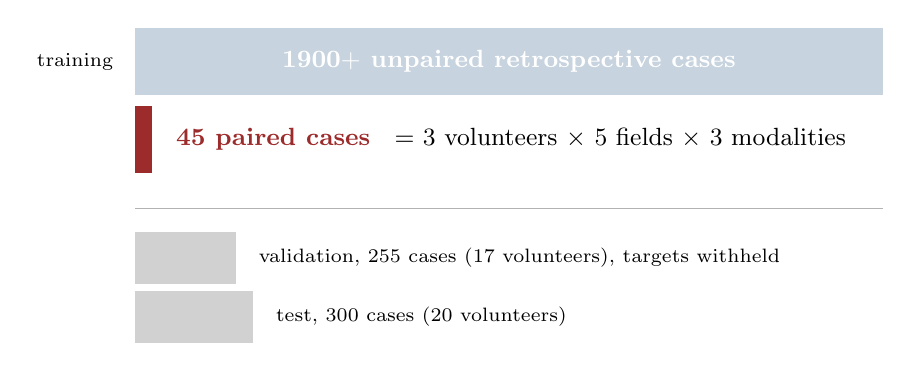
\begin{tikzpicture}[font=\small]
    \fill[accent!25] (0,0) rectangle (9.5,0.85);
    \node[font=\small, white] at (4.75,0.42) {\textbf{1900$+$ unpaired retrospective cases}};
    \node[left, font=\scriptsize] at (-0.15,0.42) {training};

    \fill[warn] (0,-1.0) rectangle (0.22,-0.15);
    \node[right, font=\small] at (0.4,-0.57) {\bad{45 paired cases} \; = 3 volunteers $\times$ 5 fields $\times$ 3 modalities};

    \draw[black!30] (0,-1.45) -- (9.5,-1.45);

    % Bar widths are on the same scale as the training bar: 9.5 cm = 1900 cases.
    \fill[black!18] (0,-2.4) rectangle (1.28,-1.75);
    \node[right, font=\scriptsize] at (1.45,-2.07) {validation, 255 cases (17 volunteers), targets withheld};
    \fill[black!18] (0,-3.15) rectangle (1.50,-2.5);
    \node[right, font=\scriptsize] at (1.67,-2.82) {test, 300 cases (20 volunteers)};
  \end{tikzpicture}

  \vspace{1.2em}
\end{frame}

% ============================================================ FINDINGS ======

\begin{frame}{Control group, Task 1}
  \ph{F}
  \parttag{ESTABLISHED IN REPORT I}

  \centering
  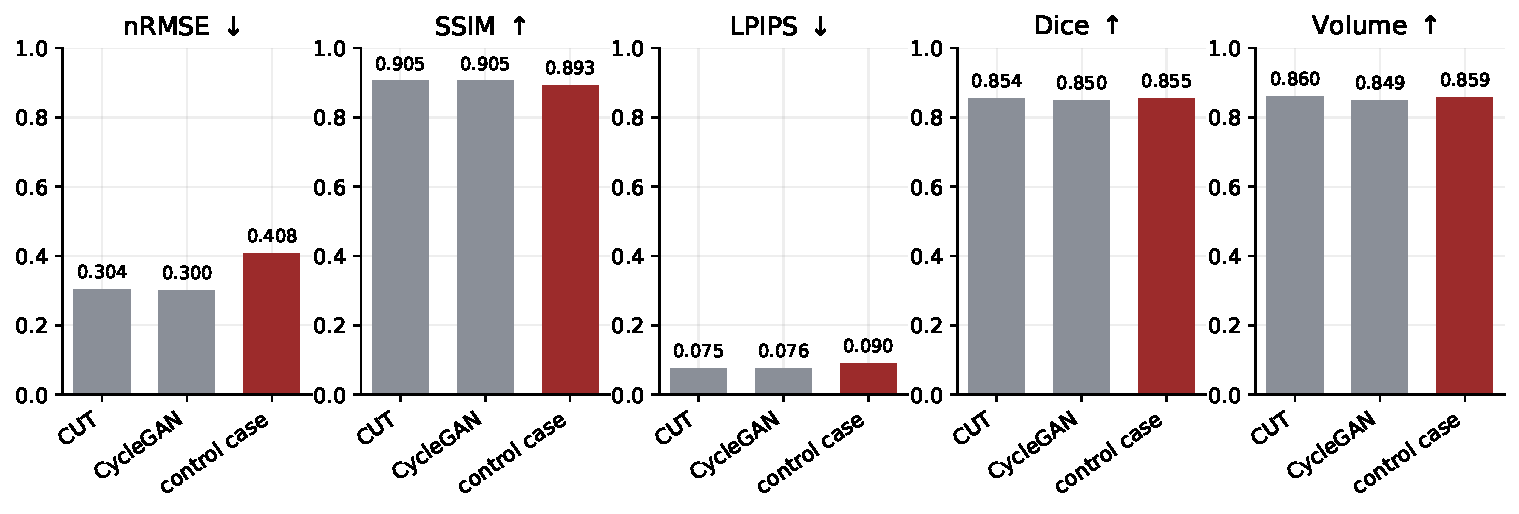
\includegraphics[width=\linewidth]{figures/slide_control_case.pdf}

  \vspace{0.6em}
  \raggedright
  \gloss{The control group returns the input volume unchanged. It is within noise of both trained
  baselines on SSIM, LPIPS, Dice and volume consistency, only losing on nRMSE, indicating a lack of performance.}
\end{frame}

\begin{frame}{Spectral exponent gap}
  \ph{D}
  \parttag{ESTABLISHED IN REPORT I}

  \centering
  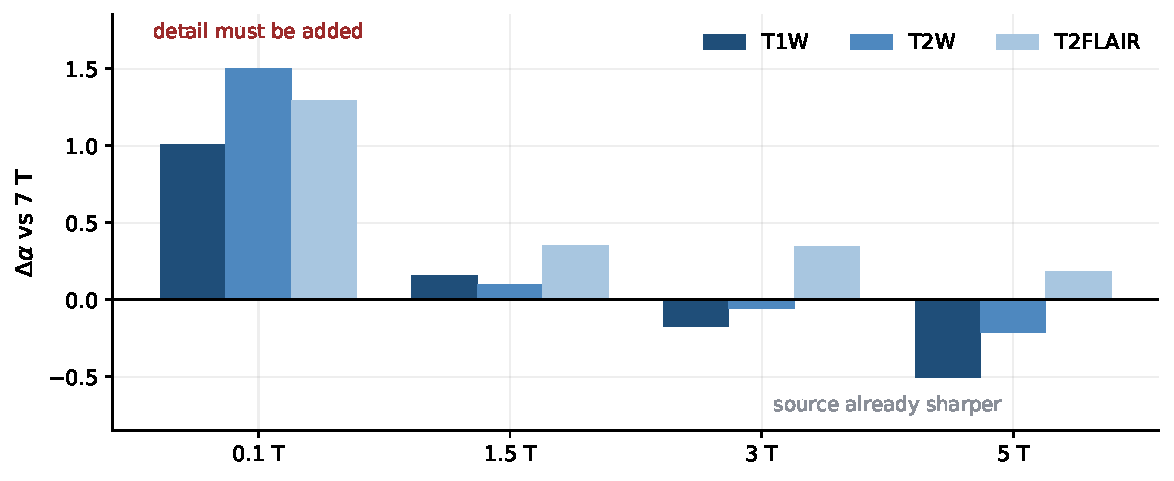
\includegraphics[width=0.86\linewidth]{figures/slide_delta_alpha.pdf}

  \vspace{0.4em}
  \raggedright
  \gloss{Power spectra follow $P(f) \propto f^{-\alpha}$. $\Delta\alpha = \alpha_{\text{source}} -
  \alpha_{7\,\mathrm{T}}$ is the HF deficit the model must close. \\
  It is substantial at 0.1\,T and near zero or negative elsewhere.}
\end{frame}

% ============================================================ DONE ==========

\begin{frame}{Constraints and solution proposals}
  \ph{D}
  \parttag{WORK SINCE REPORT I}

  \centering
  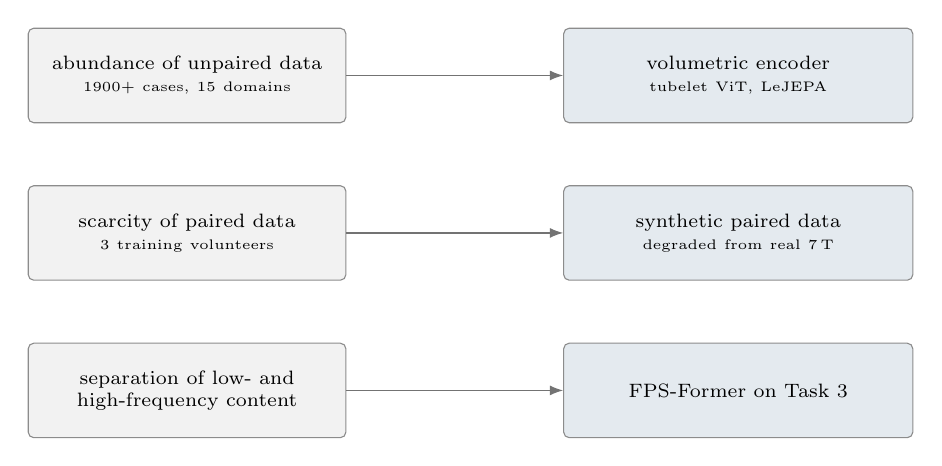
\begin{tikzpicture}[>=Latex, font=\small,
    con/.style={draw=black!45, fill=black!5, rounded corners=2pt, text width=38mm,
                align=center, minimum height=12mm, font=\scriptsize},
    res/.style={draw=black!45, fill=accent!12, rounded corners=2pt, text width=42mm,
                align=center, minimum height=12mm, font=\scriptsize}]

    \node[con] (c1) at (0,2.0)  {abundance of unpaired data\\{\tiny 1900$+$ cases, 15 domains}};
    \node[con] (c2) at (0,0)    {scarcity of paired data\\{\tiny 3 training volunteers}};
    \node[con] (c3) at (0,-2.0) {separation of low- and high-frequency content};

    \node[res] (r1) at (7.0,2.0)  {volumetric encoder\\{\tiny tubelet ViT, LeJEPA}};
    \node[res] (r2) at (7.0,0)    {synthetic paired data\\{\tiny degraded from real 7\,T}};
    \node[res] (r3) at (7.0,-2.0) {FPS-Former on Task 3};

    \foreach \a/\b in {c1/r1, c2/r2, c3/r3} \draw[->, black!55] (\a) -- (\b);
  \end{tikzpicture}
\end{frame}

\begin{frame}{Volumetric encoder}
  \ph{F}
  \parttag{WORK SINCE REPORT I}

  \centering
  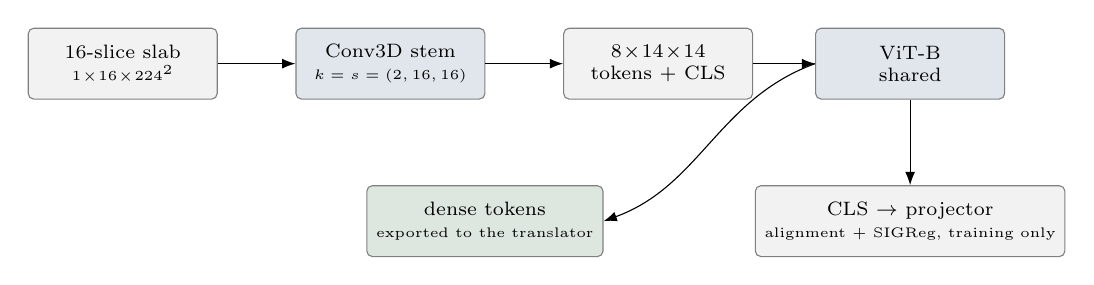
\begin{tikzpicture}[>=Latex, font=\scriptsize,
    b/.style={draw=black!50, rounded corners=2pt, align=center, minimum height=9mm,
              minimum width=24mm}]
    \node[b, fill=black!5]   (s) at (0,0)   {16-slice slab\\{\tiny $1\!\times\!16\!\times\!224^2$}};
    \node[b, fill=accent!14] (t) at (3.4,0) {Conv3D stem\\{\tiny $k=s=(2,16,16)$}};
    \node[b, fill=black!5]   (g) at (6.8,0) {$8\!\times\!14\!\times\!14$\\tokens $+$ CLS};
    \node[b, fill=accent!14] (v) at (10.0,0) {ViT-B\\shared};

    \node[b, fill=black!5, minimum width=30mm] (c) at (10.0,-2.0)
      {CLS $\rightarrow$ projector\\{\tiny alignment $+$ SIGReg, training only}};
    \node[b, fill=good!16, minimum width=30mm] (d) at (4.6,-2.0)
      {dense tokens\\{\tiny exported to the translator}};

    \foreach \a/\b in {s/t, t/g, g/v} \draw[->] (\a) -- (\b);
    \draw[->] (v) -- (c);
    \draw[->] (v.west) to[out=200, in=20] (d.east);
  \end{tikzpicture}

  \vspace{1.4em}
  % \raggedright
  % \begin{airy}
  %   \item Replaces the slice-wise encoder of Report I; slabs give through-plane context.
  %   \item \textbf{Status:} trains, loss curves stable. No downstream number. A stable loss is also
  %   consistent with a collapsed representation.
  % \end{airy}
\end{frame}

\begin{frame}{Tubelet LeJEPA training}
  \ph{F}
  \parttag{WORK SINCE REPORT I}

  \centering
  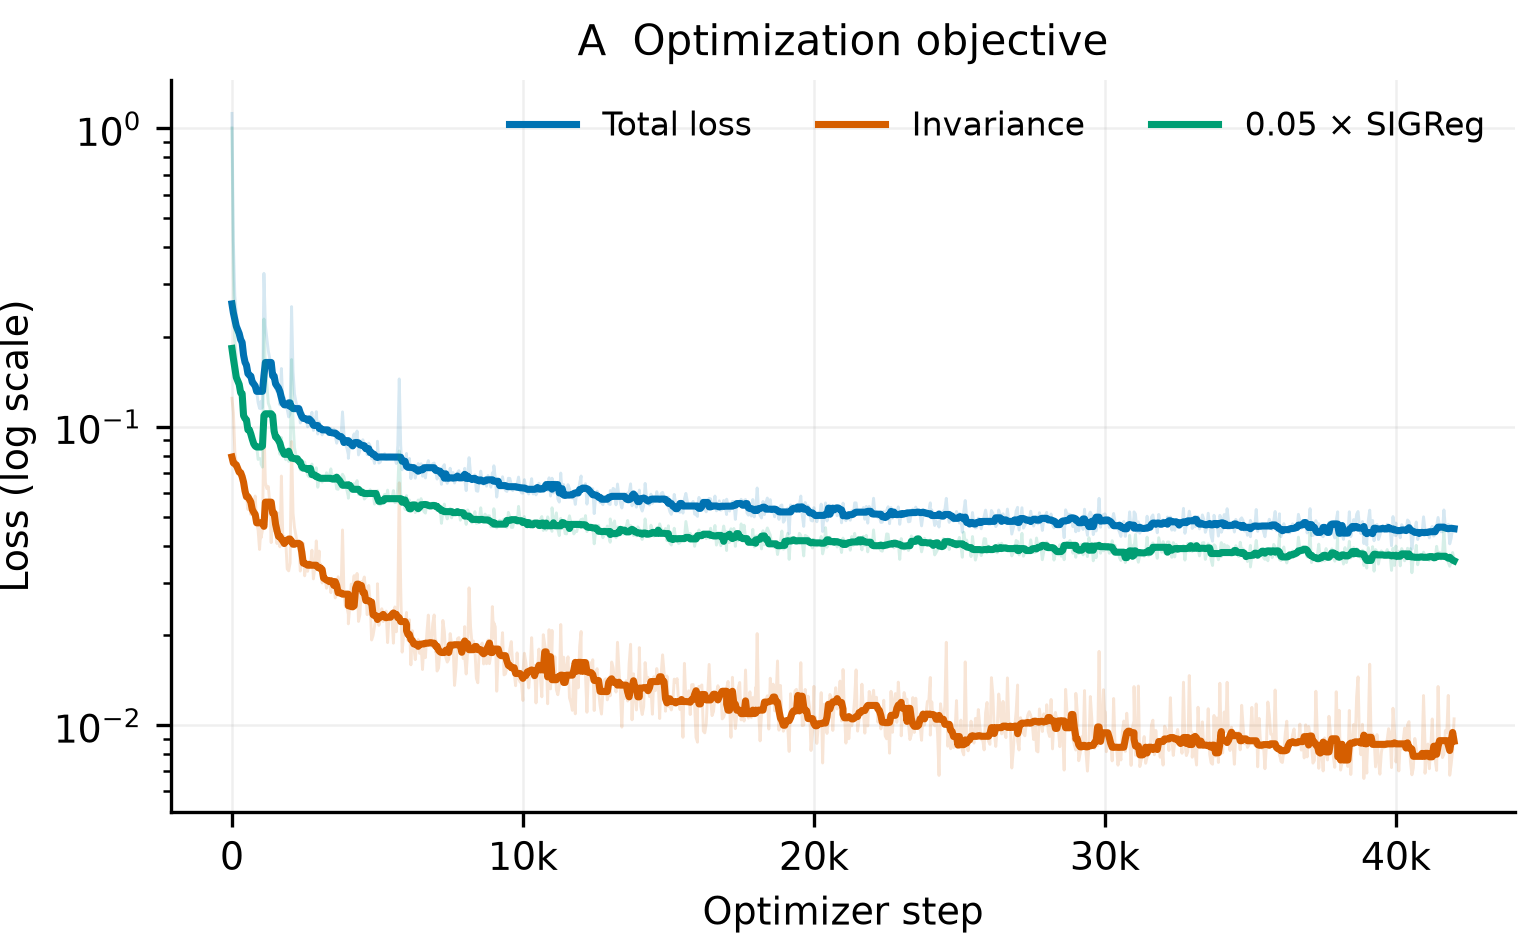
\includegraphics[height=0.68\textheight]{figures/slide_lejepa_loss.png}

  \vspace{0.2em}
  \raggedright
  \gloss{42k optimizer steps. Both terms flatten with no zero collapse.}
\end{frame}

\begin{frame}{Synthetic pair generation}
  \ph{R}
  \parttag{WORK SINCE REPORT I}

  \centering
  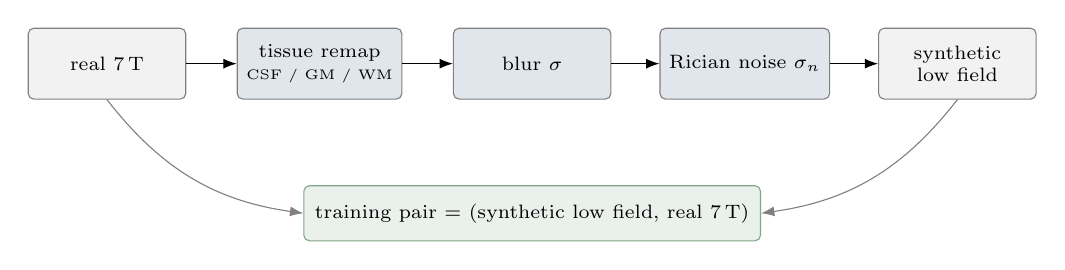
\begin{tikzpicture}[>=Latex, font=\scriptsize,
    b/.style={draw=black!50, rounded corners=2pt, align=center, minimum height=9mm,
              minimum width=20mm}]
    \node[b, fill=black!5]   (x) at (0,0)    {real 7\,T};
    \node[b, fill=accent!14] (r) at (2.7,0)  {tissue remap\\{\tiny CSF / GM / WM}};
    \node[b, fill=accent!14] (g) at (5.4,0)  {blur $\sigma$};
    \node[b, fill=accent!14] (n) at (8.1,0)  {Rician noise $\sigma_n$};
    \node[b, fill=black!5]   (y) at (10.8,0) {synthetic\\low field};
    \foreach \a/\b in {x/r, r/g, g/n, n/y} \draw[->] (\a)--(\b);

    \node[draw=good!60, fill=good!10, rounded corners=2pt, minimum width=58mm, minimum height=7mm]
      (p) at (5.4,-1.9) {training pair $=$ (synthetic low field, real 7\,T)};
    \draw[->, black!50] (x.south) to[bend right=22] (p.west);
    \draw[->, black!50] (y.south) to[bend left=22]  (p.east);
  \end{tikzpicture}

  \vspace{1.2em}
  \raggedright
  \begin{airy}
    \item Pairing exact: same anatomy, same grid.
    \item Tissue-specific remap (CSF/GM/WM), not a single global shift.
    \item Remap strength, $\sigma$ and $\sigma_n$ resampled per call, every synthetic pair is different.
  \end{airy}
\end{frame}

\begin{frame}{Synthetic output: example slice}
  \ph{R}
  \parttag{WORK SINCE REPORT I}

  \centering
  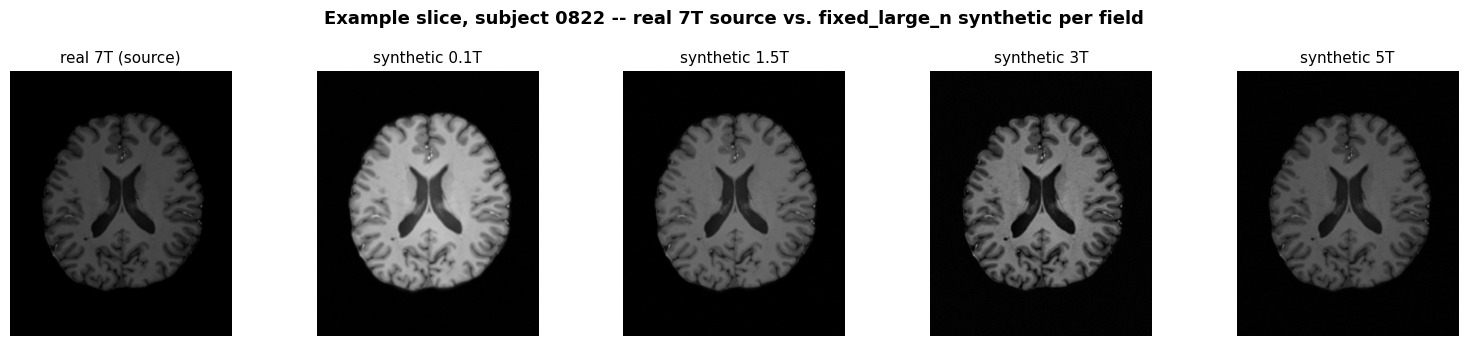
\includegraphics[width=\linewidth]{figures/synth_example_slices.png}

  \vspace{1.0em}
  \raggedright
  \gloss{One axial slice, same subject. Anatomy aimed to be preserved by construction; \\
  contrast, sharpness and noise vary.}
\end{frame}

\begin{frame}{Synthetic output: intensity distributions}
  \ph{R}
  \parttag{WORK SINCE REPORT I}

  \centering
  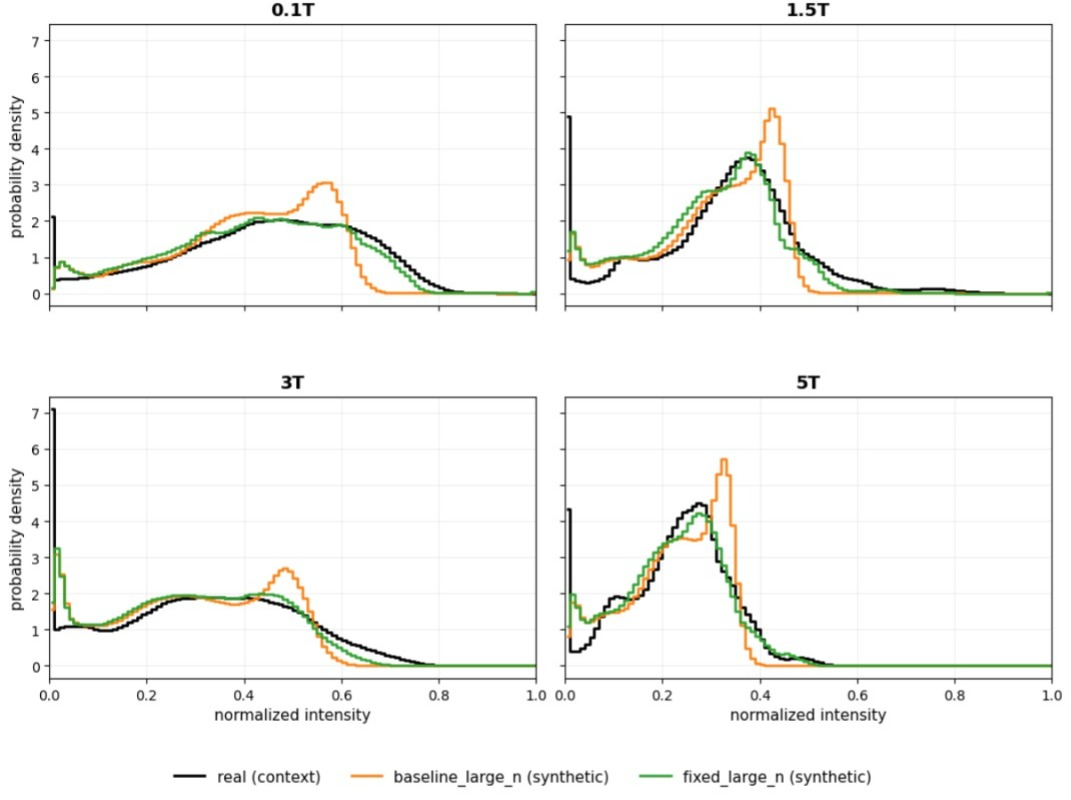
\includegraphics[height=0.68\textheight]{figures/synth_tissue_histograms.png}

  \vspace{0.2em}
  \raggedright
  \gloss{Black: real. Orange: initial generator. Green: corrected generator.}
\end{frame}

\begin{frame}{Between-volume diversity}
  \ph{R}
  \parttag{WORK SINCE REPORT I}

  \centering
  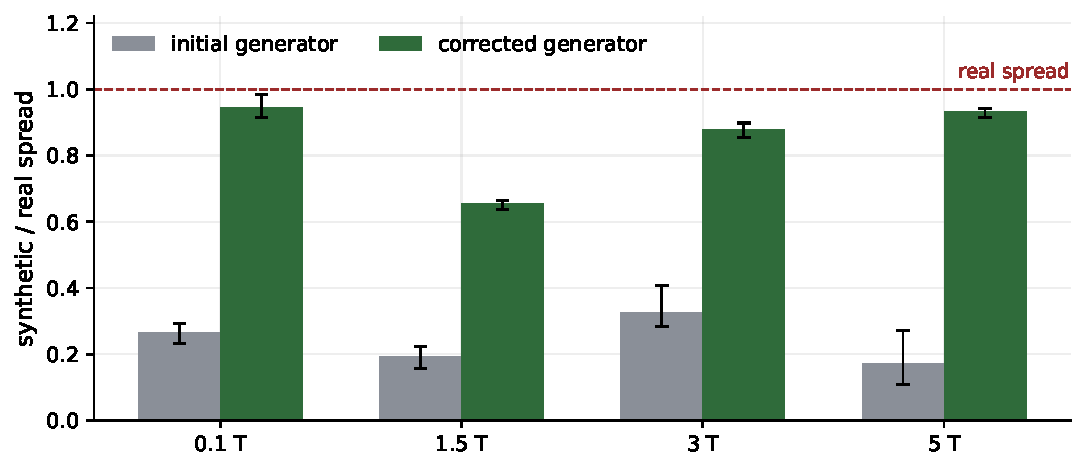
\includegraphics[width=0.80\linewidth]{figures/slide_diversity.pdf}

  \vspace{0.4em}
  \raggedright
  \gloss{Ratio of synthetic to real standard deviation of tissue means across volumes; bars are the
  mean over CSF, GM and WM, whiskers the range. The initial generator pushed every sample toward one
  average profile per field. The corrected generator varies the target profile per sample. 1.5\,T
  remains short.}
\end{frame}

\begin{frame}{Common point: separation of frequency bands}
  \ph{R+A}
  \parttag{WORK SINCE REPORT I}

  \centering
  \resizebox{\linewidth}{!}{%
  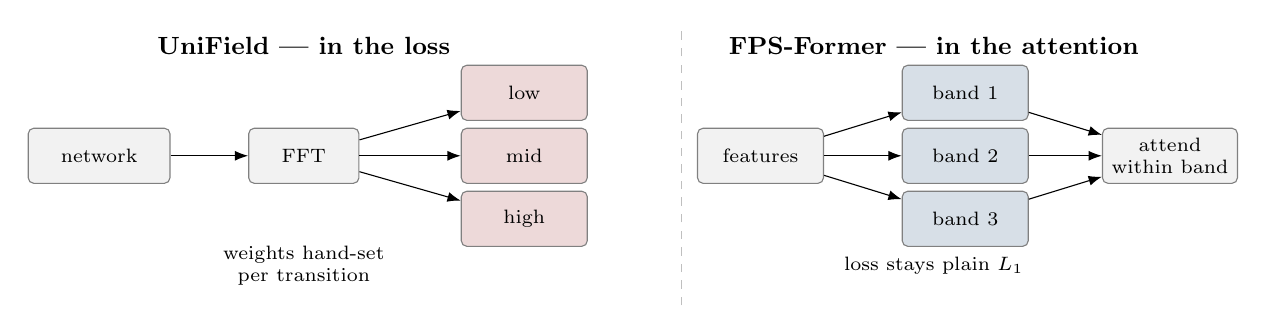
\begin{tikzpicture}[>=Latex, font=\scriptsize,
    b/.style={draw=black!50, rounded corners=2pt, align=center, minimum height=7mm}]

    \node[font=\small\bfseries, black] at (2.6,2.3) {UniField --- in the loss};
    \node[b, fill=black!5, minimum width=18mm]   (n1) at (0,0.9)  {network};
    \node[b, fill=black!5, minimum width=14mm]   (f1) at (2.6,0.9) {FFT};
    \node[b, fill=warn!18, minimum width=16mm]   (bl) at (5.4,1.7) {low};
    \node[b, fill=warn!18, minimum width=16mm]   (bm) at (5.4,0.9) {mid};
    \node[b, fill=warn!18, minimum width=16mm]   (bh) at (5.4,0.1) {high};
    \draw[->] (n1)--(f1);
    \foreach \b in {bl,bm,bh} \draw[->] (f1) -- (\b);
    \node[font=\scriptsize, align=center] at (2.6,-0.5) {weights hand-set\\per transition};

    \draw[black!25, dashed] (7.4,-1.0) -- (7.4,2.5);

    \node[font=\small\bfseries, black] at (10.6,2.3) {FPS-Former --- in the attention};
    \node[b, fill=black!5, minimum width=16mm] (f2) at (8.4,0.9) {features};
    \node[b, fill=accent!18, minimum width=16mm] (t1) at (11.0,1.7) {band 1};
    \node[b, fill=accent!18, minimum width=16mm] (t2) at (11.0,0.9) {band 2};
    \node[b, fill=accent!18, minimum width=16mm] (t3) at (11.0,0.1) {band 3};
    \node[b, fill=black!5, minimum width=14mm] (a2) at (13.6,0.9) {attend\\within band};
    \foreach \t in {t1,t2,t3} { \draw[->] (f2) -- (\t); \draw[->] (\t) -- (a2); }
    \node[font=\scriptsize, align=center] at (10.6,-0.5) {loss stays plain $L_1$};
  \end{tikzpicture}}

  \vspace{1.2em}
  \raggedright
  \gloss{Similar ideas, different approaches. Measured $\Delta\alpha$ is the quantity UniField's band
  weights approximate by hand. \\
  It changes sign above 1.5\,T, so a single fixed weighting seems not appropriate.}
\end{frame}

\begin{frame}{Task 3 results}
  \ph{A}
  \parttag{WORK SINCE REPORT I}

  \centering
  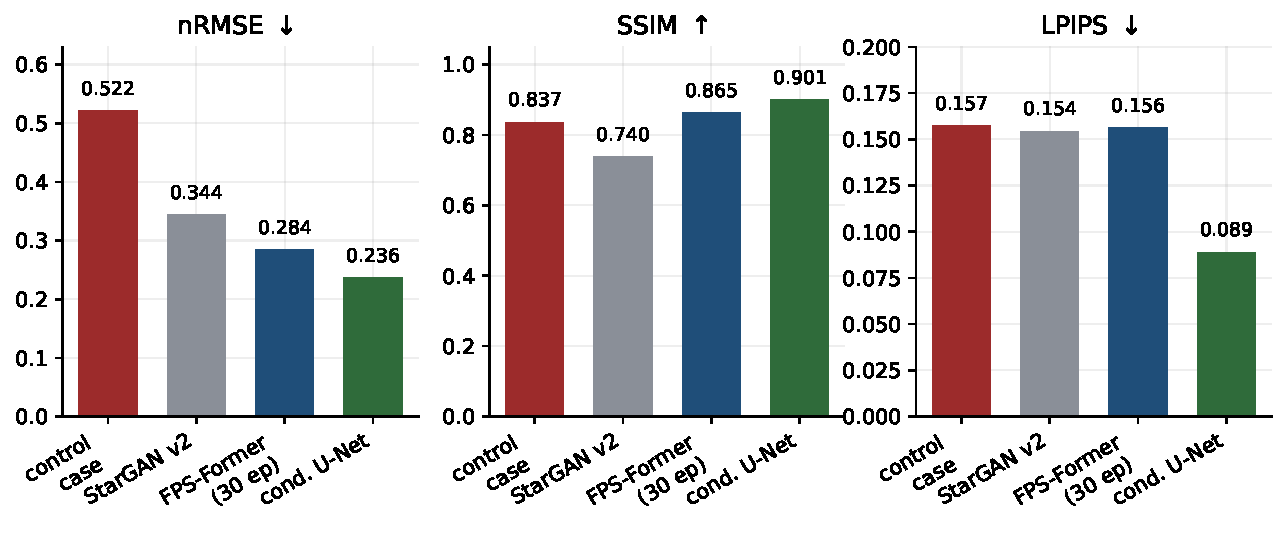
\includegraphics[width=0.86\linewidth]{figures/slide_task3.pdf}

  \vspace{0.4em}
  \raggedright
  \gloss{All modality-averaged. The control group is the unmodified input, scored on the platform. \\
  On LPIPS all three trained models sit within 0.003 of it, and FPS-Former improves on it by 0.0011. \\
  Control group also beats the challenge baseline on SSIM. Only the conditional U-Net separates itself on
  every metric.}
\end{frame}

\begin{frame}{Task 3 predictions, every source field to 7\,T}
  \ph{A}
  \parttag{WORK SINCE REPORT I}

  \centering
  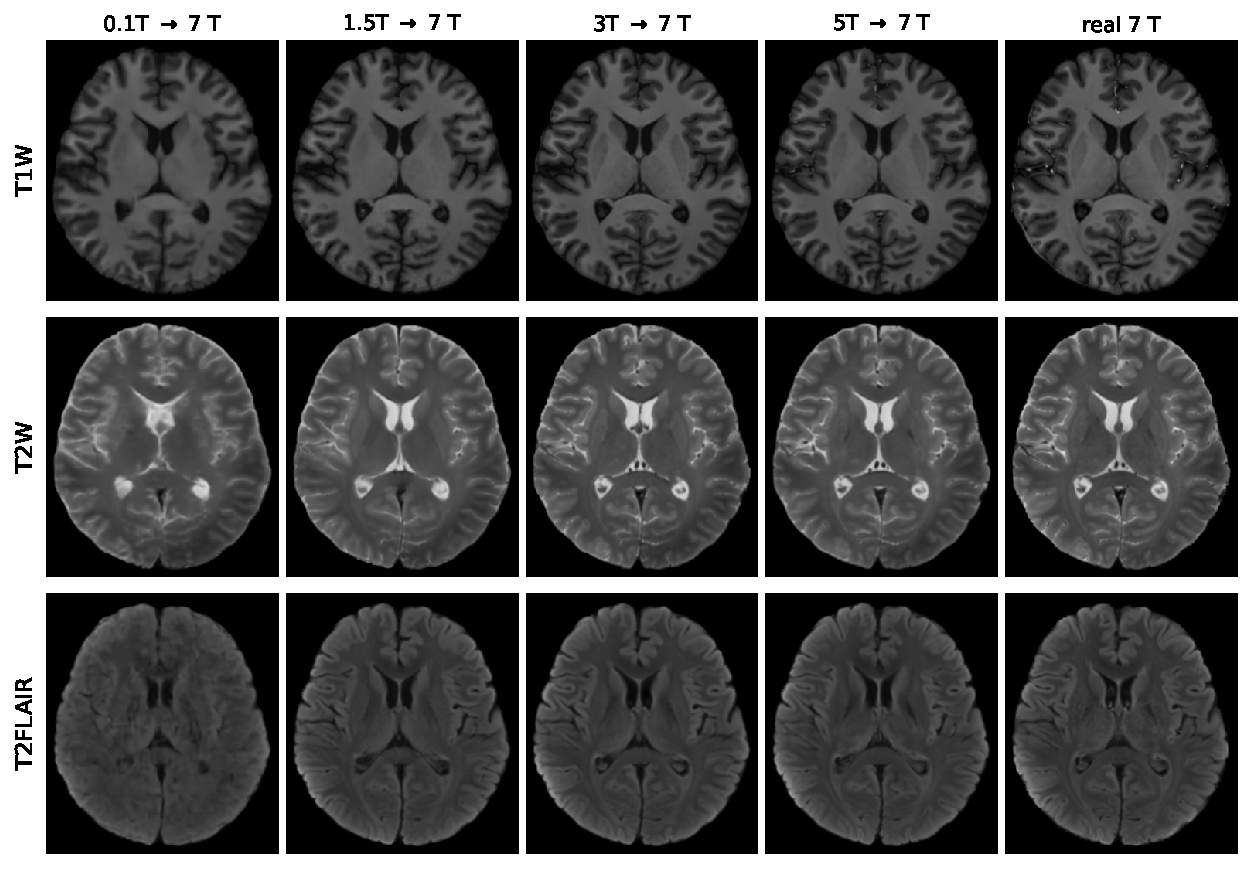
\includegraphics[height=0.66\textheight]{figures/slide_task3_sweep.pdf}

  \vspace{0.2em}
  \raggedright
  \gloss{Same subject and slice throughout; last column is the 7\,T. 
  In-sample: this subject is in the paired split the checkpoint was fine-tuned on.}
\end{frame}

\begin{frame}{Task 3 predictions against ground truth, 0.1\,T $\rightarrow$ 7\,T}
  \ph{A}
  \parttag{WORK SINCE REPORT I}

  \centering
  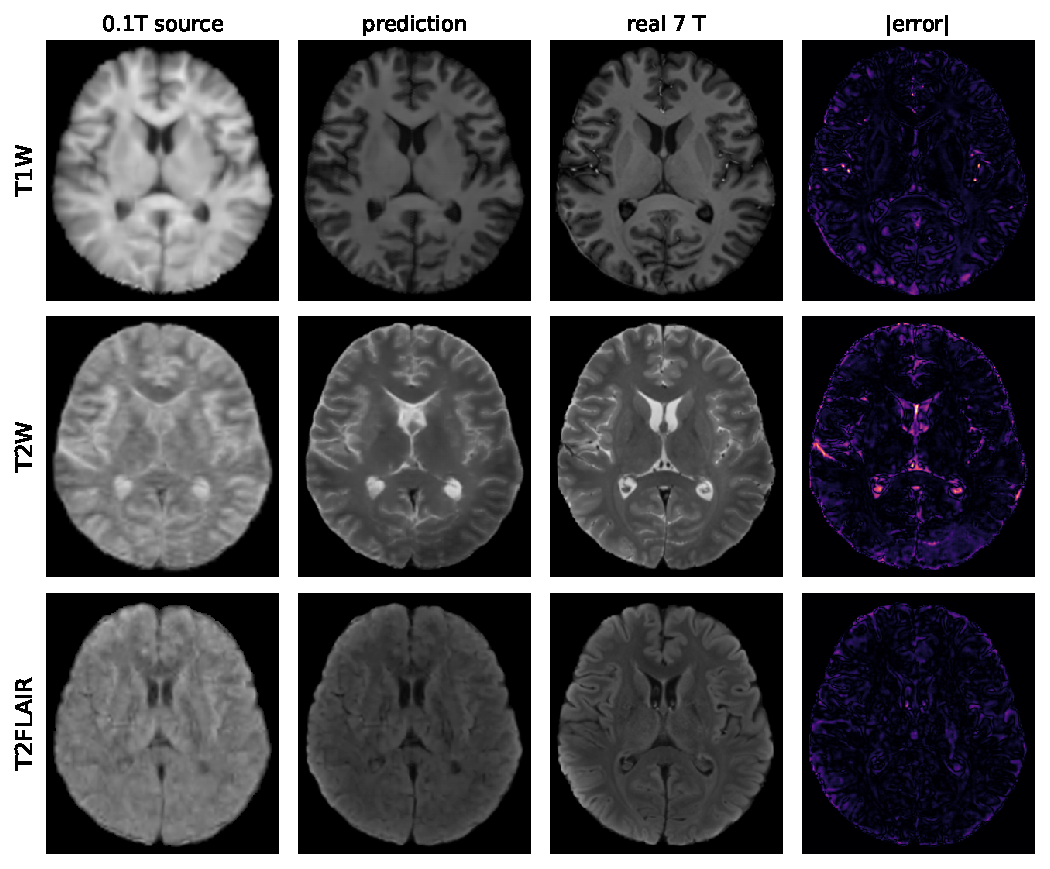
\includegraphics[height=0.64\textheight]{figures/slide_task3_gt.pdf}

  \vspace{0.2em}
  \raggedright
  \gloss{Transition with the largest $\Delta\alpha$. Error is structured on
  edges and vessels rather than spread over tissue, which is what a loss of fine detail looks like.
  In-sample, as above.}
\end{frame}

\begin{frame}{Status}
  \ph{D}
  \parttag{WORK SINCE REPORT I}

  \vspace{0.8em}
  \footnotesize
  \begin{tabular}{@{}l@{\hspace{7mm}}l@{\hspace{7mm}}l@{}}
    \toprule
    \textbf{Done} & \textbf{Comments} & \textbf{Keep Track} \\
    \midrule
    Pretrained volumetric encoder
      & optimisation is stable
      & does it transfer? \\[0.35em]
    Synthetic data generation
      & it matches the real spread
      & pretraining benefits? \\[0.35em]
    FPS-Former training
      & no LPIPS gain over control group
      & keep or drop it? \\
    \bottomrule
  \end{tabular}

  \vspace{1.4em}
\end{frame}

% ============================================================ NEXT ==========

\begin{frame}{Stages 1--2 as a conditioned experiment}
  \ph{D}
  \parttag{NEXT \quad suggestion}

  \centering
  \vspace{0.4em}
  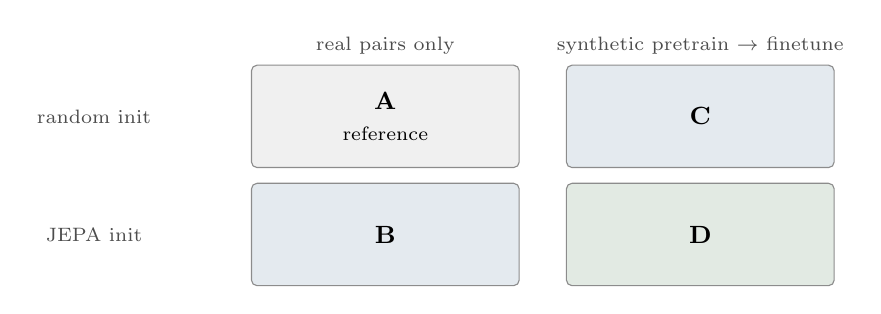
\begin{tikzpicture}[font=\small,
    c/.style={draw=black!45, rounded corners=2pt, minimum width=34mm, minimum height=13mm,
              align=center}]
    \node[font=\scriptsize, black!70] at (2.2,1.55) {real pairs only};
    \node[font=\scriptsize, black!70] at (6.2,1.55) {synthetic pretrain $\rightarrow$ finetune};
    \node[font=\scriptsize, black!70, align=right] at (-1.5,0.65) {random init};
    \node[font=\scriptsize, black!70, align=right] at (-1.5,-0.85) {JEPA init};

    \node[c, fill=black!6]   (A) at (2.2,0.65)  {\textbf{A}\\{\scriptsize reference}};
    \node[c, fill=accent!12] (C) at (6.2,0.65)  {\textbf{C}};
    \node[c, fill=accent!12] (B) at (2.2,-0.85) {\textbf{B}};
    \node[c, fill=good!14]   (D) at (6.2,-0.85) {\textbf{D}};
  \end{tikzpicture}

  \vspace{1.2em}
  \raggedright
  \begin{airy}
    \item $B - A$: value of the encoder alone. \quad $C - A$: value of the synthetic data alone.
    \item $D - C$ against $B - A$: does the encoder still help once synthetic pretraining is in place?
  \end{airy}

  \gloss{Four runs of a cheap model. $D - C \approx B - A$ means the two act independently; \\
  $D - C \approx 0$ means the encoder is redundant once the synthetic data is there.}
\end{frame}

\begin{frame}{Stage 3 candidates}
  \ph{D}
  \parttag{NEXT}

  \begin{airy}
    \item \textbf{Band-weighted loss.} Spectral term on the same U-Net, per-band weights derived from
    the measured $\Delta\alpha$, conditioned on the transition.
    \item \textbf{Reconsider conditioning.} Currently adding domain embedding at the bottleneck only;
    source--target difference lives at fine scales. \\
    Considering a modulation scheme that can act at multiple layers of size.
    \item \textbf{FPS-Former, schedule matched} to the U-Net --- or dropped.
  \end{airy}

  \vspace{1.0em}
  \gloss{All three are edits to a model that already exists.}

  \srcline{reports/progress\_report\_2.pdf \quad mrixfields.chihucloud.com/2026}
\end{frame}

\begin{frame}
  \vfill
  \centering
  {\Large\bfseries Thank you}

  \vspace{1.0em}
  {\small Questions?}
  \vfill
\end{frame}

\end{document}
